\documentclass{article}
\setcounter{secnumdepth}{-1}
\usepackage{graphicx}
\usepackage{amsfonts}
\usepackage{amsmath}
\usepackage[margin=0.9in, paperwidth=8.5in, paperheight=11in]{geometry}
\begin{document}
\title{S.I.E.V.E. Progress Report}
\author{Wayne Yang \\ Nick Kullman \\ Graham Clenaghan}
\date{Spring 2015}
\maketitle

\section{Sieve Analysis for Vaccine Trials}


\section{Sequence Data Visualization Tools}

There are several existing tools for the visualization of genomic / proteomic sequence data.  Some of these tools tend to provide a very detailed display of the alignments of sequences for a particular gene / protein from multiple patients.  While this approach allows a user to see all of their data at once, it does not provide quick and easy analysis of particular sites in the sequence across patients or subsets of patients.  The following example is from a software called Aliview CITATION HERE.

\begin{center}
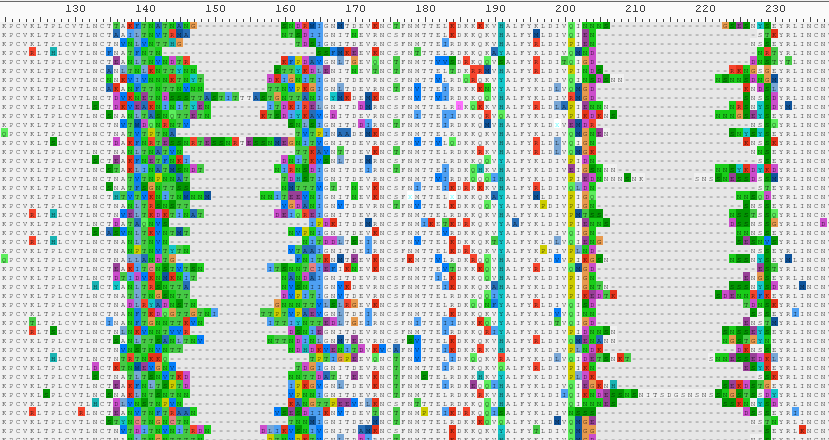
\includegraphics[height=3in,width=4in]{aliview.png}
\end{center}
Clearly, understanding the pattern of mutations and any relationships to treatment status for a particular site in the sequence is very difficult to do in this view with any precision.
\\
\newline
\noindent Other tools are geared towards specific analyses

\section{Project Plan}

\end{document}

http://www.ncbi.nlm.nih.gov/pubmed/25095880